\section{Methodology}
The purpose of this study is to determine whether through gamification and off-the-shelf hardware and an automated feedback, telemetry-driven system, a user can be trained as a race driver. This chapter describes the research methodology of this study, describes the procedure used to set up the experiment for data collection and provides an explanation of the procedures used to analyse the collected data.

\subsubsection{Research methodology}
The research has applied both an experimental and descriptive methodology, one complimenting the other. In order to be able to derive trust worth conclusion from the experiment, it was imperative to minimize any bias between the experimental and controlled groups, by ensuring the groups are roughly equivalent at the beginning of the study. Once the independent variable is applied and change in behaviour between the groups is noted, the difference can be confidently attributed solely to the introduction of the independent variable given it can be assumed group equivalence. The possibility exists, however, that the differences we observe at the end of the study are due to the fact that the groups of participants differ at the start of the experiment even before they receive one level or another of the independent variable. Thus it was assured by means of simple random group assignment the initial equivalence of the groups prior to the introduction of the independent variable\cite{introductiontobehavioralresearchmethods}.

Moving on to the descriptive methodology part in which questionnaires over an interviews were preferred. This choice was based literature suggesting questionnaires being less expensive and easier to administer than personal interviews. they lend themselves to group administration; and, they allow confidentiality to be assured. Although interviews give the chance for a participant to better explain them self, having users fill in questionnaires on their own creates a sense of anonymity which encourages users to be more truthful\cite{introductiontobehavioralresearchmethods}. 

\subsection{Experiment Setup}
It was important for the experiment setup to be able to make participants feel as if they are driving a real car, yet being able to keep within the constraints of the budget which aims to use of off the shelf, consumer affordable items. Furthermore, any environment variables had to be controlled as much as possible in order to avoid any inherited bias ending favouring a particular participant.

\subsubsection{Environment}
Ensuring all participants were exposed to the same testing environment allowed to have any bias to be introduced. Distractions could have played a major role in a participant's performs. As such the experiments have been carried out in a closed room, free from any noise from crowds. One participant at a time was allowed in the room, this avoid having other participants gaing any information from other participants' experiments while also avoiding participants distracting each other. The room which was used for the experiments had two walls with windows facing the out side which in the morning had sun light come in directly, in cases potentially temporally blinding a participant during an experiment. To avoid this, the setup was moved to a location in the room in which sun rays did not effect participants during any time of the day,
	
\subsubsection{Hardware}
With hardware being the most expensive part of this research, it was important to be able to find a good balance between cost and and quality. In this case quality refers to the ability a piece of hardware has to convey the sense of realism to a participant. Starting off with the steering wheel set, it had to be able to turn as much as a race car wheel and be able to accurately replicate the forces a race car steering wheel experiences during use. This is done through force feedback technology, which allows participants to better feel what the car is doing. An H shifter and pedals were also required. Shifters don't vary much, as force feedback technology is not implemented in these devices, however it was important to use an H shifter as this is what most participants are expected to be familiar with this type. Moving on the pedals, there are sets which try to replicate varying pressure for brake and clutch pedals using hydraulic actuated pistons which is what one expects to find in a real car. These pedals set are very good and replicating the force one is required to use while braking or activating the clutch, however these are very expensive and as such fail out of budget. As such a more entry level set has been used which still performs well.
The steering and other mentioned peripherals were attached to a home made racing rig, which was built using the seating position one would experience in a race car, this is typical a low seating position the steering wheel and shifter close to the driver. In addition a racing seat off a local race car has been fitted with the aim of giving further sense of immersion to participants by using and replicating properties a race driver experiences.\\
With virtual reality being introduced in recent years and gaining traction, it was looked at as a possibility as means to integrate it into the system. During initial testing virtual reality was proving to an important component, helping users get completed immersed into the simulator. However, users were getting dizzy and some had eye irritation. Furthermore, Oculus dropped support for Windows 10, which was the operating system used for this project, this compromised the headset reliability and as a result virtual reality had to be abounded.

<Insert comparison chart here and say something about it>

\subsubsection{Software}
The last part of the experiment setup tackles the to driving model, which has been simulated by a consumer available off the shelf sim-racing game called Assetto Corsa which is widely accepted by world wide sim racers as being a valid sim racing game which simulates the real world accurately. Assetto Corsa provides realistic car handling and characteristics vehicle models and real life racing tracks. The tracks are laser scanned, this technology manages to replicate a track surface accurately allowing this project ensure the track being used is as close as possible to the real track. In addition, Assetto Corsa also provides the fucntionality to disable any damage, wear and tear of the car, which allows for better constant variables as cars will not get progsivley worse during a session hindering a participants. Although there are other sim racing games which provide the same level of realism such as Project Cars and iRacing, Assetto Corsa has the advantage of an easy to use telemetry API which any programming language can access and a strong community of developers who can help should one need assistance on the API use.

<Insert comparison chart here and say something about it>

\subsection{Feedback System}
	The feedback system will relies heavily on the quality of telemetry data it can get. In order to achieve this, the data has to be, ordered, supplied in real time, accurate and carry enough information for feedback to be generated. As such the feedback processing is multi thread and also designed to run as part of a distributed system. The telemetry data is kept in main memory for fast access during processing from which each thread can read from. This allows any loaded feedback modules to be able to carry out their respective analysis before the next telemetry data is received. This is especially important as if a modules takes to long to process it will lag behind resulting in the feedback being given too late, rendering it inaccurate. In addition any telemetry data which is received is append to a log file. This log file is used to run through a session off-line, allowing for further data analysis for the evaluation section of this report. The log is the primary way to validate the hypothesis put forward during the project.
	During initial prototypes for the feedback system, feedback was conveyed using a heads up display approach, however this proved to be too distracting for users, furthermore there where issues trying to provide meaningful feedback by means of text or pictures on screen overlayed over the sim game. Users found the feedback hard to interpret at a glance. The heads up display was changed in favour of an auditory feedback, as it is less introduce\cite{leahy2003auditory}. It would have been interesting to look into a hybrid approach in which auditory feedback is aided with heads up display. This might have been especially beneficial in cases in which the feedback needed to convey degrees or ranges. However, due to time constraints it wsa settled to have an sole auditory system. 

\begin{figure}[!htb]
	\centering
	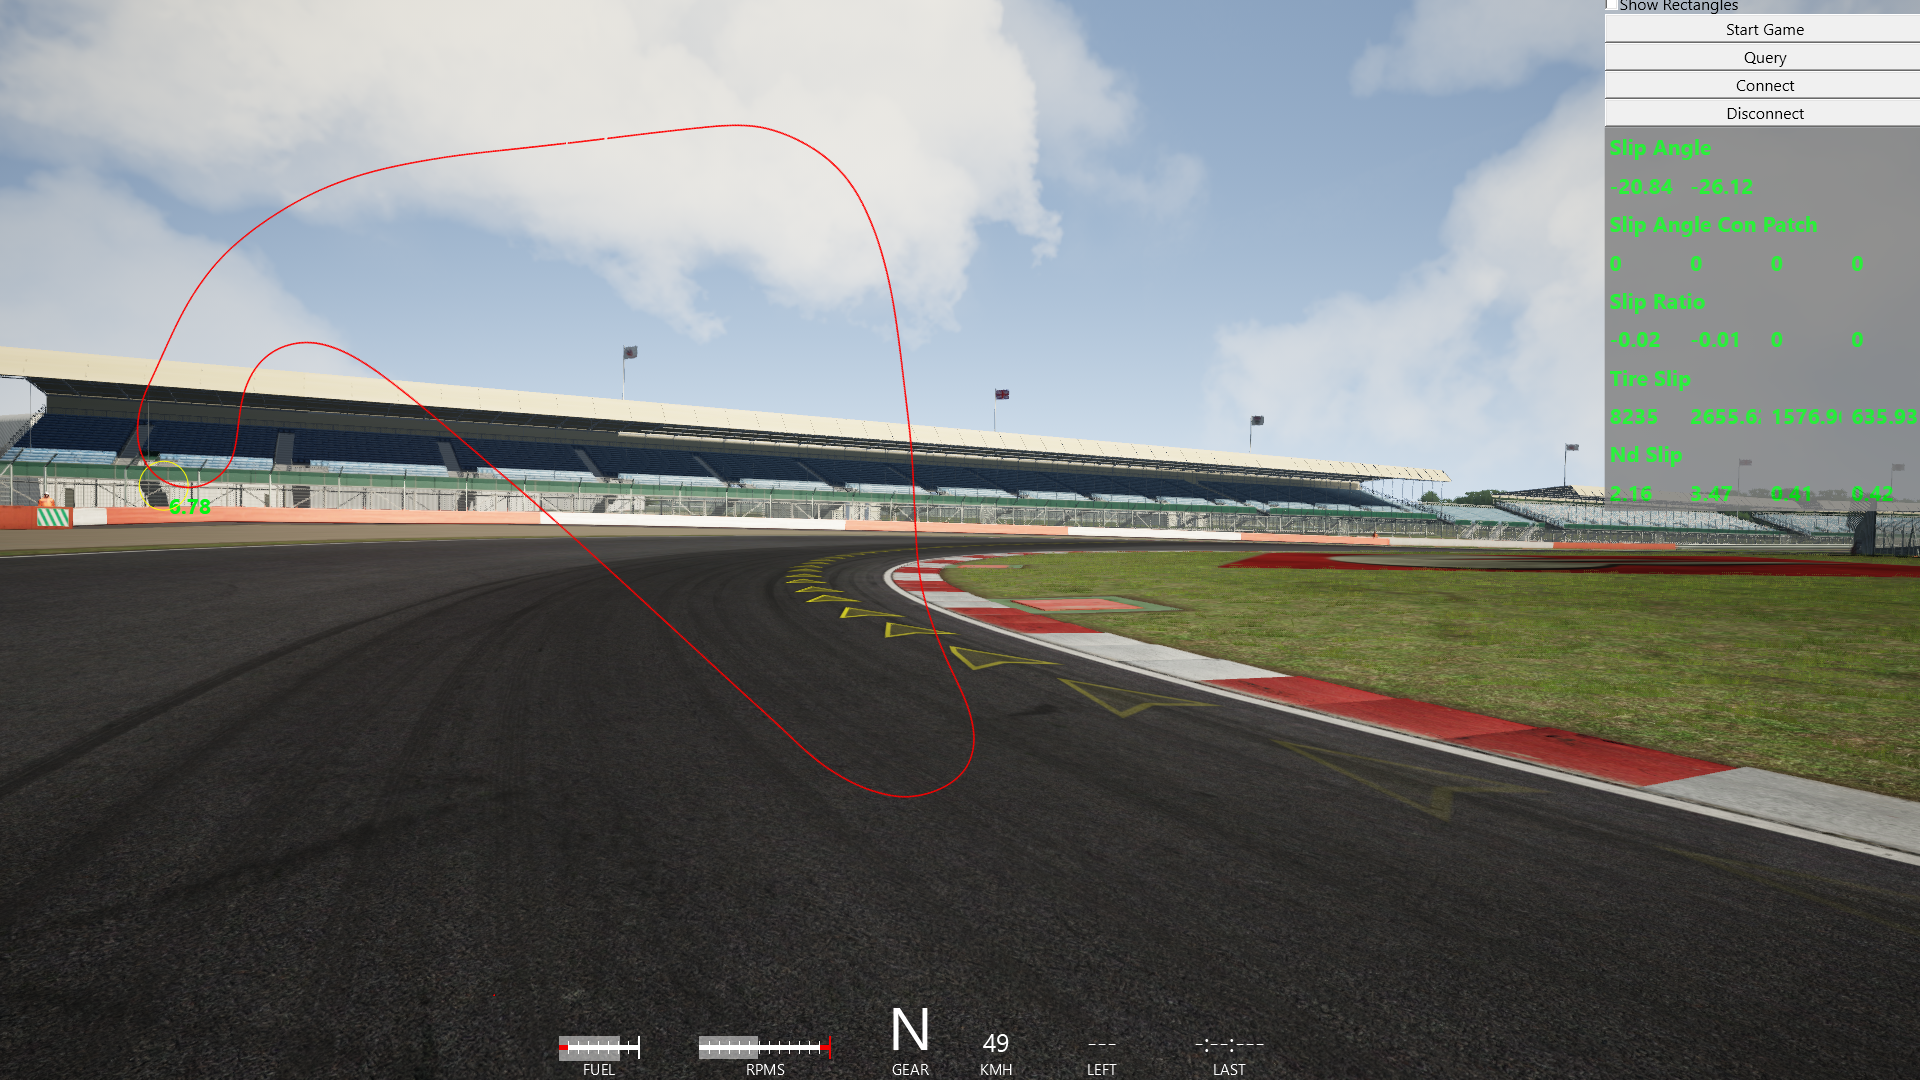
\includegraphics[height=7cm]{images/uiPrototype}
	\caption{Early feedback system heads up display prototype}
	\label{fig:uiPrototype}
\end{figure}

\subsection{Evaluation}

\subsubsection{Experiment structure}
	In order to evaluate the effectiveness of the system a user study needs to take place. Participants are to be split randomly into two groups. One group will be referred as the feedback group, the other will be referred to as the base group. All participants, regardless of in which group they have been assigned, will be given one hour slots in which they are asked to race around a track. The one hour slots are to be divided in sub sessions to be carried out in the following order. Five minutes to get the rig setup and adjusted for the participant. This might require having to move the seat further back or forward in order for the participant to be more comfortable. By having two separate groups using the same setup and being allocated the same time, it is possible to determine if any improvements are due to the feedback system teach the users, or users getting better on their on by practicing. If there is a statistical significant differnce showing the feedback group  improves 
	During the experiments participants will also be asked to fill in a pre-experiment survey, be given information about the racing rig usage and care, and how the one hour slot is divided. Ten minutes of driving are then carried out, the aim of this session is to allow the participant to get familiar with the rig, track and car. Once the first session of driving is carried out the participant is told in which group he/she has been assigned. The participant is also shown a picture of a typical race line through a corner and a brief explanation is given. This is done to make it easier on the feedback group to better understand the auditory race line feedback which might be given. As for the base group, the same picture and information are given out as to have both groups provided with the same information and ensuring any learning is done by means of the feedback system. Another ten minutes of driving follow, with the same setup as the previous one which gives participants the chance to keep practicing and improving. A final five minutes of driving will take place, during this session no one will have the feedback system enabled. The aim of this session is to give the participant a final chance to improve upon his/her time. in addition for the feedback group, data from the last five minutes could point out if the participant was able to learn any techniques and use them with out being given further feedback. Finally the participant is given the post survey to fill in.

\subsubsection{Track and Car choice}
The track and car choice is to made based on suggestion from the literature review. The car should not be too powerful as it would be harder to control. Another characteristic to take into account is whether to choose a front wheel drive or a rear wheel drive one. Rear wheel drive cars tend to be less predictable in corners, while front wheel ones tend to understeer more resulting in more predictable cornering which in turn makes front wheel drive easier to drive. The track should be as flat and smooth as possible. This makes it easier to drive the circuit as an uneven surface may upset the car making it lose control. The track also needs to have wide run off areas. these areas are located along the circuit where racers are most likely to unintentionally depart from the prescribed course. This gives the racers time to slow down before colliding with walls.

\subsubsection{Data Collection and Sampling}
	Participants will be accepted from any background and level of relevant experience. Two survey are required,  a pre experiment survey will be designed with the aim of collecting demographic user data. Given these data it will be possible to identify any data cluster which might form. The data is too include three sections, personal, driving history and games and motorsport history. The personal section will simple collect the participant's gender and age, and driving history relates to a participant's vehicle driving experience in the real world. Games and motorsport history relates to the any exposure or first hand experience a participant might have had with racing video games or real life motorsports event. From this survey is it expected to answer questions such as, if this project is more beneficial to a specific group of participants having a common background and if real life experience with driving makes it easier for a participant to use a sim racing game. \\
	After the experiment takes place another qualitative survey will be handed out. This survey will focus on gathering feedback from the participant point of view. Here it is of interest to gather how the participant feels about the racing rig setup, did it feel real? and was it comfortable? Furthermore, participants will be given a chance to comment about the experiment set-up, track and car choice and the time allocations. From this it will be possible to determine if participants found the setup to meet the objectives a seroius game should achieve. The feedback group will be asked to fill in an extra section asking for their impressions on the feedback system. This section will mostly focusing on trying to understand if participants felt the feedback system was helpful and if there is something which can be improved upon. The participants responses will be mapped to the telemetry data from which responses can be validated. In the case participants feel the feedback is not accurate, feedback is not helpful, comments can be correlated back to the telemetry data.\\
	During the sessions, telemetry data will be logged and stored for off line analysis for the evaluation. The main data which are of interests to this project are lap times. Decreasing lap times are give a good indication of the participant's skill and performance improvements. The analysis needs to focus on clustering the data into two main groups, the base group and the feedback group, from these the best lap time of each user is to be considered for each session. The aim is to find any statistical difference in the rate of improvement between the base group and the feedback group. However as much as the ultimate goal is to improve the lap time, one must first improve on specific skills. It is possible for a participant to improve on a skill area while hindering another. In such case it would be interesting to analyse the telemetry data from which it could be determined if a participant did improve or hinder certain areas which could explain why lap times did not improve or get worst.
	Once the experiments are all carried out, the data will be loaded into a database management system which will make it easier to query and extract relevant data. Such as exporting a report of the lap times of a user rather than having all the data points along the laps. The extracted data will then be loaded into as statistical analysis software from which mean variance test can be carried out on the base group and feedback group. From this tests it will be ultimately possible to determine if the experiment did manage to help the participants in the feedback group to improve their skills and lap times.